\subsection{Zustandshaltung der Pipeline}

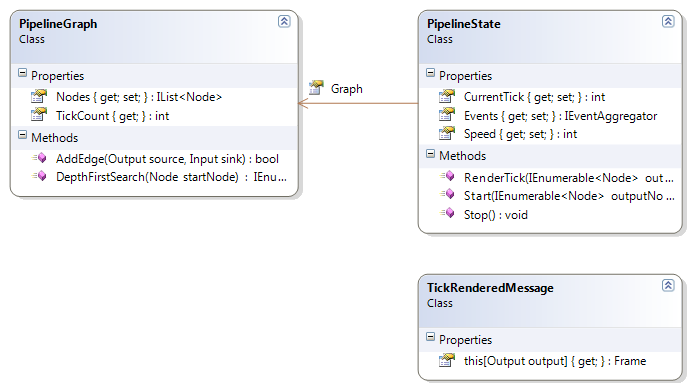
\includegraphics[width=\textwidth]{YuvKA.Pipeline/states.png}
Diese Gruppe von Klassen dient dazu, den Zustand der Pipeline zu verwalten. Der \name{PipelineState} benutzt zur Verwaltung der im Pipeline-Graphen vorhandenen Knoten und Kanten den \name{PipelineGraph}. Er ist zudem dafür zuständig die Berechnung der Pipeline zu starten und zu stoppen. Die \name{FrameRenderedMessage} wird geworfen, wenn ein Zeitabschnitt berechnet ist.

\subsubsection{YuvKA.Pipeline.PipelineState}

\begin{verbatim}
[DataContract]
public class PipelineState
\end{verbatim}

\paragraph{Beschreibung}~\\
Die Klasse \name{PipelineState} vereint in sich den Gesamtzustand des Datenmodells, womit durch ihre Serialisierung alle relevanten Programmdaten gespeichert werden. Sie enthält den aktuellen Wiedergabestatus und bietet zur Wiedergabe eine Schnittstelle zum \name{PipelineDriver}.

\paragraph{Typmember}
\begin{itemize}

\property{Tick}
	\begin{verbatim}
	[DataMember]
	public int Tick { get; set; }
	\end{verbatim}
	Ruft den Index des zuletzt berechneten \name{Tick}s ab oder legt ihn fest. Das Neusetzen führt nicht zum erneuten Berechnen der im Tick berechneten \name{Frame}s, sondern muss mit \name{Start} explizit angefordert werden. Ein \name{Tick} repräsentiert hierbei den Zeitaschnitt für die Berechnung aller relevanten \name{Frame}s mit dem gegebenen Index.

\property{Speed}
	\begin{verbatim}
	[DataMember]
	public int Speed { get; set; }
	\end{verbatim}
	Ruft die Abspielgeschwindigkeit in Frames pro Sekunde ab oder legt sie fest.

\property{Graph}
	\begin{verbatim}
	[DataMember]
	public PipelineGraph Graph { get; }
	\end{verbatim}
	Ruft den \name{PipelineGraph} ab, der die Struktur der Pipeline repräsentiert, oder legt ihn fest.

\property{Events}
	\begin{verbatim}
	[Import(typeof(IEventAggregator))]
	public IEventAgggregator Events { get; set; }
	\end{verbatim}
	Per Dependency Injection injizierte Schnittstelle zum Caliburn Message System, über das die Ausgabefenster über die Beendigung aller im aktuellen Tick berechneten \name{Frame}s benachrichtigt werden.



\method{Start}
	\begin{verbatim}
	public void Start()
	\end{verbatim}
	Weist den \name{PipelineDriver} an, die Pipeline ab dem aktuellen \name{Tick} zu berechnen. Bei abgeschlossener Berechnung aller \name{Frame}s im aktuellen Zeitabschnitt wird eine \name{FrameRenderedMessage} geworfen.

\method{Stop}
	\begin{verbatim}
	public void Stop()
	\end{verbatim}
	Beendet die Wiedergabe und stoppt den \name{PipelineDriver}. Danach vom \name{PipelineDriver} asynchron erhaltene \name{Frame}s werden ignoriert.
\end{itemize}

\subsubsection{YuvKA.Pipeline.PipelineGraph}
	
\begin{verbatim}
[DataContract]
public class PipelineGraph	
\end{verbatim}

\paragraph{Beschreibung}~\\
Die Klasse \name{PipelineGraph} verwaltet den Aufbau des Pipeline-Graphen. 
	
\paragraph{Typmember}
\begin{itemize}

\property{Nodes}
	\begin{verbatim}
	[DataMember]
	public IList<Node> Nodes { get; }
	\end{verbatim}
	Verwaltet die im Pipeline-Graphen verfügbaren Knoten und gibt sie ab.

\property{FrameCount}
	\begin{verbatim}
	[DataMember]
	public int FrameCount { get; }
	\end{verbatim}
	Ruft die maximale Länge aller als Input gegebenen Videos ab.


	
\method{AddEdge}
	\begin{verbatim}
	public bool AddEdge(Output source, Input sink)
	\end{verbatim}
	Wenn die durch \name{source} und \name{sink} spezifizierte Kante zu keinem Zyklus innerhalb des Pipeline-Graphen führt, so soll sie durch setzen der Output-Property von \name{source} als \name{sink} hinzugefügt und true ausgegeben werden. Andernfalls soll die Kante nicht zum Graphen hinzugefügt und false ausgegeben werden.
\end{itemize}
	
\subsubsection{YuvKA.Pipeline.FrameRenderedMessage}
		
\begin{verbatim}
public class FrameRenderedMessage
\end{verbatim}

\paragraph{Beschreibung}~\\
Die Klasse \name{FrameRenderedMessage} enthält die im letzten Tick berechneten \name{Frame}s aller \name{Output}s.

\paragraph{Typmember}
\begin{itemize}
	
\property{this[]}
	\begin{verbatim}
	public Frame this[Output output] { get; }
	\end{verbatim}
Indexer. Ruft den durch \name{output} spezifizierten \name{Frame} auf.

\end{itemize}




	


